\section{Introduction to implementation}
This report explains our implementation of the project. \\
Overall the project uses the classes seen in Figure \ref{fig:UMLClassDiagram}

\begin{figure}[h!]
\centering
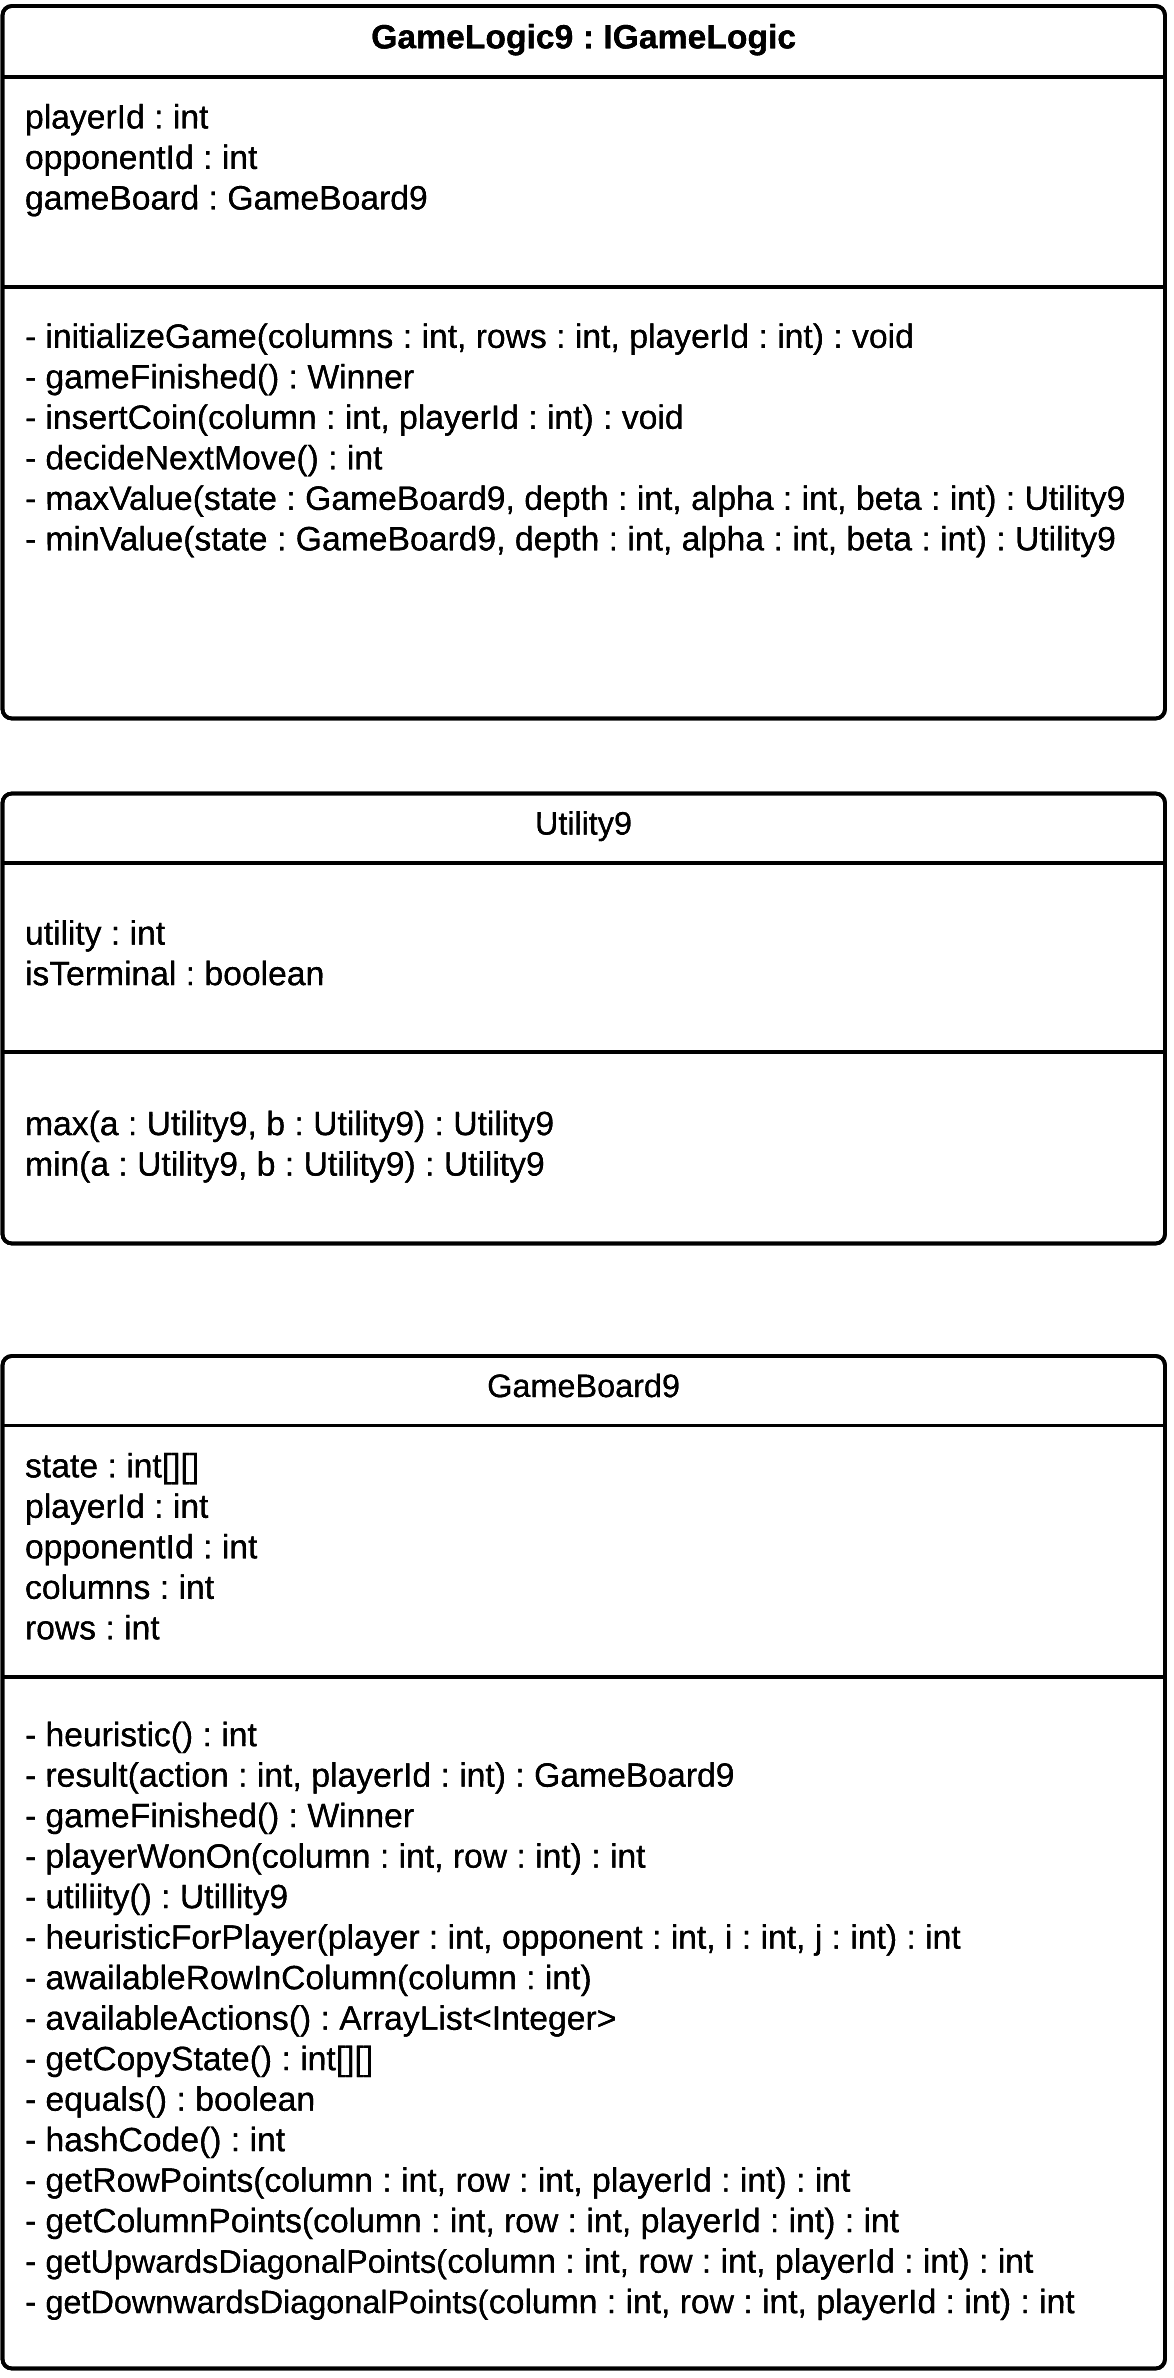
\includegraphics[width=0.65\linewidth]{ClassDiagram.png}
\caption{UML class-diagram showing off classes implemented by group \label{fig:UMLClassDiagram}}
\end{figure}

The class \texttt{Utility9} is used to represent utility. The functions \texttt{maxValue} and \texttt{minValue} returns \texttt{Utility9} instances. It has two fields; \texttt{utiliity} to represent some utility, and a flag, \texttt{isTerminal} stating whether this is a terminal state or not. \\
Moreover, \texttt{Utility9} provides two static methods, \texttt{max(...)} and \texttt{min(...)}, that takes as arguments two \texttt{Utility9} instances, and returns the largest and the smallest, respectively; determined by comparing their utility-values. 

The \texttt{Gameboard9} class is used to encapsulate logic in relation to (the state of) and operations on the gameboard. 

\subsection{Evaluation and cut-off function}

Turning our attention to \texttt{GameLogic9}'s method, \texttt{decideNextMove()}, we initially extract our available actions, i.e. what columns we can fill in "coins". These actions are now explored within a set time-threshold (10 seconds) \textit{and} in increasing depth, untill time runs out. We continously search for a highest utility, \texttt{currentBest}; if the utility for the current action (in the current depth) exceeds the current highest utility, \texttt{currentBest} is updated. $\alpha$ is updated to whoever's largest of $\alpha$ (initially set to $-\infty$) and \texttt{utility}.




\subsection{$\alpha$-$\beta$ pruning}